In the each of the following exercises, find the coordinates of the focus, axis of the parabola, the equation of the directrix and the length of the latus rectum.
\begin{enumerate}[label=\thesubsection.\arabic*,ref=\thesubsection.\theenumi]
\item $y^2$=12x 
\label{chapters/11/11/2/1}
\\
\solution
%%See 
\tabref{tab:std-conic-params-sol}
and 
\figref{fig:11/11/2/1Fig1}.
\begin{figure}[!h]
	\begin{center}
		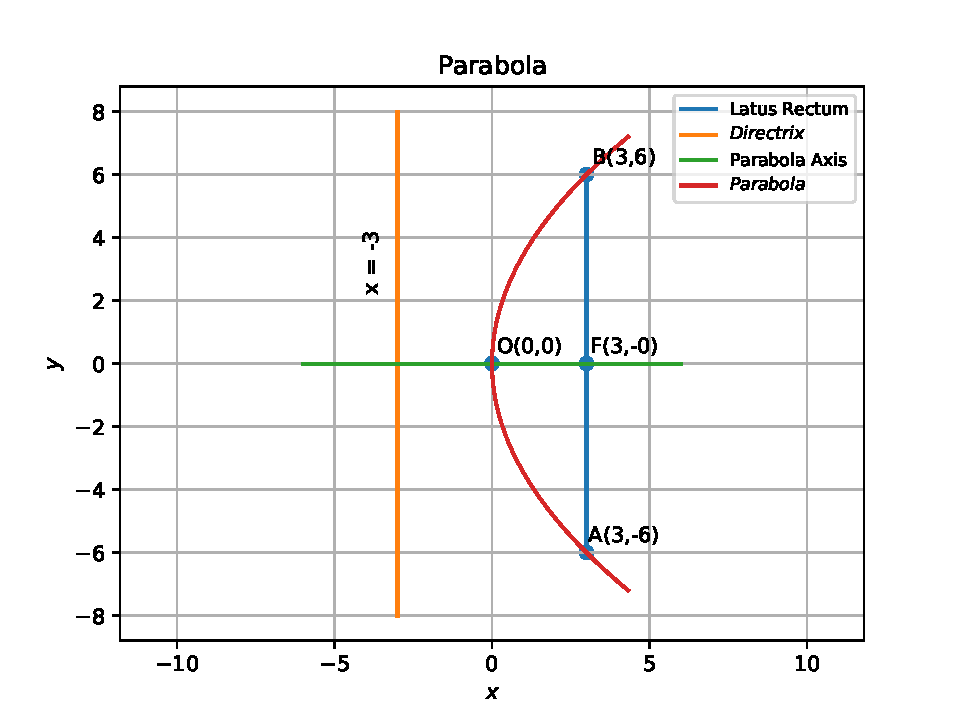
\includegraphics[width=\columnwidth]{chapters/11/11/2/1/figs/problem1.pdf}
	\end{center}
\caption{}
\label{fig:11/11/2/1Fig1}
\end{figure}

\item $x^2$=6y 
\\
\solution
%%\iffalse
\documentclass[12pt]{article}
\usepackage{graphicx}
\usepackage{amsmath}
\usepackage{mathtools}
\usepackage{gensymb}

\newcommand{\mydet}[1]{\ensuremath{\begin{vmatrix}#1\end{vmatrix}}}
\providecommand{\brak}[1]{\ensuremath{\left(#1\right)}}
\providecommand{\norm}[1]{\left\lVert#1\right\rVert}
\newcommand{\solution}{\noindent \textbf{Solution: }}
\newcommand{\myvec}[1]{\ensuremath{\begin{pmatrix}#1\end{pmatrix}}}
\let\vec\mathbf

\begin{document}
\begin{center}
\textbf\large{CONIC SECTIONS}

\end{center}
\section*{Excercise 11.2}

Q2.Find the coordinates of the focus, axis of the parabola, the equation of the directrix and the length of the latus rectum of a parabola whose equation is given by $x^2=6y$.

\solution
\fi
The given equation of the parabola can be rearranged as
\begin{align}
	\label{eq:chapters/11/11/2/2/parabolaEq1}
	x^2-6y=0
\end{align}
The above equation can be equated to the generic equation of conic sections
\begin{align}
	\label{eq:chapters/11/11/2/2/parabolaEq2}
	g\brak{\vec{x}}=\vec{x}^\top \vec{V}\vec{x}+2\vec{u}^\top \vec{x}+f=0
\end{align}
Comparing the coefficients of both equations \eqref{eq:chapters/11/11/2/2/parabolaEq1} and \eqref{eq:chapters/11/11/2/2/parabolaEq2}
\begin{align}
	\label{eq:chapters/11/11/2/2/eqV}
	\vec{V} &= \myvec{1&0\\0&0}\\
	\label{eq:chapters/11/11/2/2/eqU}
	\vec{u} &= -\myvec{0\\3}\\
	\label{eq:chapters/11/11/2/2/eqF}
	f &= 0
\end{align}
\begin{enumerate}
\item From equation \eqref{eq:chapters/11/11/2/2/eqV}, since $\vec{V}$ is already diagonalized, the Eigen values $\lambda_1 \text{ and } \lambda_2$ are given as
\begin{align}
	\label{eq:chapters/11/11/2/2/eqEigen1}
	\lambda_1 &= 1\\
	\label{eq:chapters/11/11/2/2/eqEigen2}
	\lambda_2 &= 0
\end{align}
And the corresponding eigen vector matrix $\vec{P}$ is indentity, so the Eigen vector $\vec{p}_2$ corresponding to Eigen value $\lambda_2$ is
\begin{align}
	\vec{p}_2 &= \myvec{0\\1}\\
	\vec{n} &= \sqrt{\lambda_1}\vec{p}_2\\
		&= \sqrt{1}\myvec{0\\1}\\
		&= \myvec{0\\1}
\end{align}
Now,
\begin{align}
	\label{eq:chapters/11/11/2/2/eqC}
	c = \frac{\norm{\vec{u}}^2 - \lambda_1 f}{2\vec{u}^\top \vec{n}}
\end{align}
Substituting values of $\vec{u},\vec{n},\lambda_1 \text{ and } f$ in \eqref{eq:chapters/11/11/2/2/eqC}
\begin{align}
	c = \frac{3^2-1\brak{0}}{-2\myvec{0&3}\myvec{0\\1}} = -\frac{3}{2}
\end{align}
The focus $\vec{F}$ of parabola is expressed as
\begin{align}
	\vec{F} &= \frac{ce^2 \vec{n}-\vec{u}}{\lambda_1}\\
		&= \frac{-\frac{3}{2}\brak{1}^2 \myvec{0\\1}+\myvec{0\\3}}{1}\\
		&= \myvec{0\\\frac{3}{2}}
\end{align}
\item Equation of directrix is given as
\begin{align}
	\vec{n}^\top \vec{x} &= c\\
	\myvec{0&1}\vec{x} &= -\frac{3}{2}
\end{align}
\item The equation for the axis of parabola passing through $\vec{F}$ and orthogonal to the directrix is given as
\begin{align}
	\label{eq:chapters/11/11/2/2/eqM}
	\vec{m}^\top \brak{\vec{x}-\vec{F}} = 0
\end{align}
where $\vec{m}$ is the normal vector to the axis and also the slope of the directrix. Now since
\begin{align}
	\vec{n} = \myvec{0\\1}\\
	\vec{m} = \myvec{1\\0}
\end{align}
Substituting in \eqref{eq:chapters/11/11/2/2/eqM}
\begin{align}
	\myvec{1&0}\myvec{\vec{x}-\myvec{0\\\frac{3}{2}}}&=0\\
	\myvec{1&0}\vec{x} &= 0
\end{align}
\item The latus rectum of a parabola is given by
\begin{align}
	l&=\frac{\eta}{\lambda_1}\\
	 &=\frac{2\vec{u}^\top \vec{p}_2}{\lambda_1}\\
	 &=\frac{2\myvec{0&3}\myvec{0\\1}}{1}\\
	 &=6 \text{ units }
\end{align}
See Fig. \ref{fig:chapters/11/11/2/2/Fig1}
\begin{figure}[!h]
	\begin{center} 
	    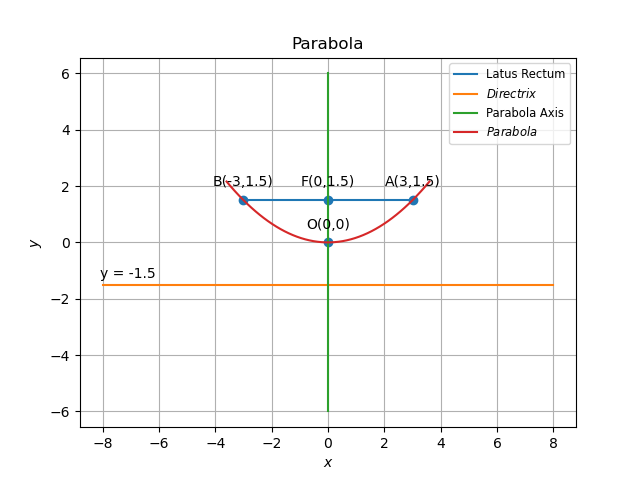
\includegraphics[width=\columnwidth]{chapters/11/11/2/2/figs/parabola}
	\end{center}
\caption{}
\label{fig:chapters/11/11/2/2/Fig1}
\end{figure}
\end{enumerate}





\item 
$y^2 = –8x$
\\
\solution
%%See \tabref{tab:std-conic-params-sol} and 
\figref{fig:chapters/11/11/2/3/1}.
\begin{figure}[H]
\centering
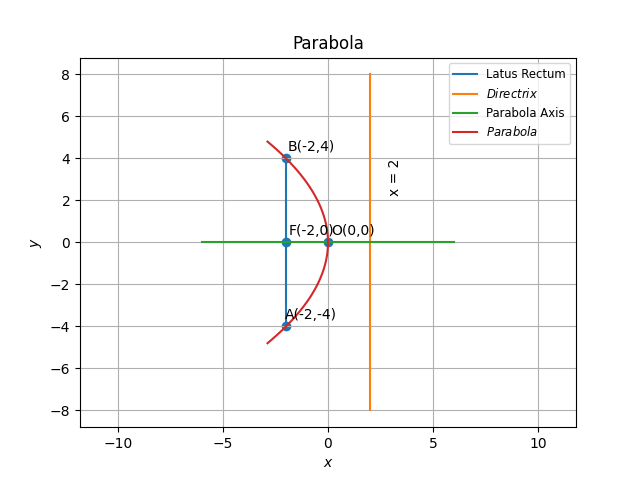
\includegraphics[width=0.75\columnwidth]{chapters/11/11/2/3/figs/fig.png}
\caption{Graph}
\label{fig:chapters/11/11/2/3/1}
\end{figure}

\item $y^2$=-8x

\item $x^2$=-16y
\\
\solution
%%See \tabref{tab:rot-conic-params-sol}
and 
\figref{fig:chapters/11/11/2/4/Fig1}.
\begin{figure}[!h]
	\begin{center} 
	    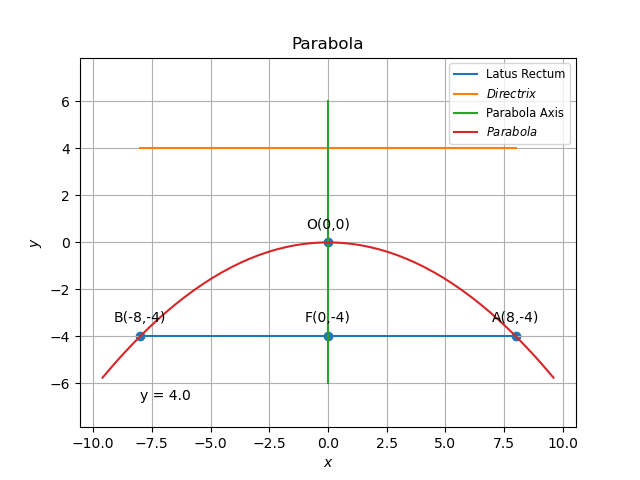
\includegraphics[width=\columnwidth]{chapters/11/11/2/4/figs/parabola}
	\end{center}
\caption{}
\label{fig:chapters/11/11/2/4/Fig1}
\end{figure}


\item $y^2$=10x  

\item $x^2$=-9y  
  \item $\frac{x^2}{36}+\frac{y^2}{16}=1$
\\
\solution
%See 
\tabref{tab:std-conic-params-sol}
and 
\figref{fig:chapters/11/11/3/1/Fig1}.
\begin{figure}[H]
	\begin{center}
		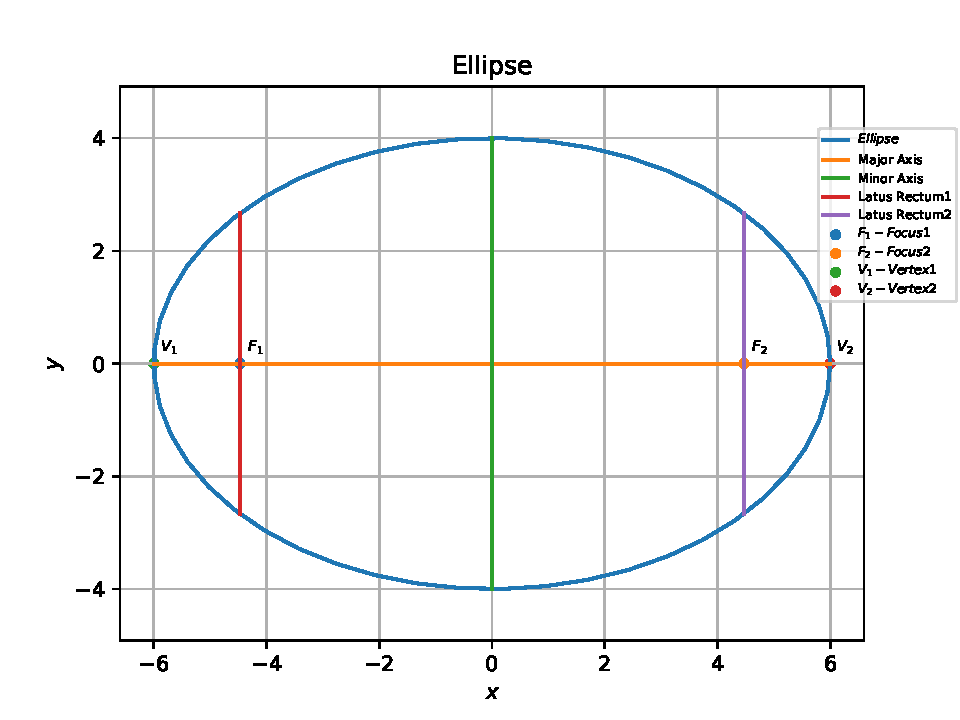
\includegraphics[width=0.75\columnwidth]{chapters/11/11/3/1/figs/problem1.pdf}
	\end{center}
\caption{}
\label{fig:chapters/11/11/3/1/Fig1}
\end{figure}

  \item $\frac{x^2}{4}+\frac{y^2}{25}=1$
\\
\solution
%The equation of the given ellipse can be rearranged as 
\begin{align}
	\label{eq:chapters/11/11/3/2/eq1}
	25x^2+4y^2-100=0
\end{align}
The above equation can be equated to the generic equation of conic sections
\begin{align}
	\label{eq:chapters/11/11/3/2/eq2}
	g\brak{\vec{x}}=\vec{x}^\top \vec{V} \vec{x} + 2\vec{u}^\top \vec{x} + f = 0
\end{align}
Comparing coefficients of both equations \eqref{eq:chapters/11/11/3/2/eq1} and \eqref{eq:chapters/11/11/3/2/eq2}
\begin{align}
	\label{eq:chapters/11/11/3/2/eq3}
	\vec{V} &= \\
	\vec{u} &= \vec{0}\\
	f &= -100
\end{align}
From equation \eqref{eq:chapters/11/11/3/2/eq3}, since $\vec{V}$ is already diagonalized, the eigen values $\lambda_1 \text{ and } \lambda_2$ are given as
\begin{align}
	\lambda_1 &= 25\\
	\lambda_2 &= 4
\end{align}
Since the given matrix $\vec{V}$ is diagonal, the Eigen vector matrix will be identity. It is given as
\begin{align}
	\vec{P} &= \myvec{\vec{p}_1 & \vec{p}_2}\\
		&= \myvec{1&0\\0&1}
\end{align}
\begin{enumerate}
\item The eccentricity of the ellipse is given as
\begin{align}
	e &= \sqrt{1 - \frac{\lambda_2}{\lambda_1}} = \sqrt{1-\frac{4}{25}}\\
	  &= \frac{\sqrt{21}}{5}
\end{align}
\item Finding the coordinates of Focii
\begin{align}
	\vec{n} &= \sqrt{\lambda_1}\vec{p}_2= \sqrt{25} \myvec{0\\1}\\
	&= \myvec{0\\5}
\end{align}
\begin{align}
	\label{eq:chapters/11/11/3/2/eq4}
	c &= \frac{e\vec{u}^\top \vec{n} \pm \sqrt{e^2 \brak{\vec{u}^\top \vec{n}}^2-\lambda_1 \brak{e^2 -1}\brak{\norm{\vec{u}}^2-\lambda_1 f}}}{\lambda_1 e\brak{e^2-1}}
\end{align}
Substituting values of $e,\vec{u},\vec{n},\lambda_1 \text{ and } f$ in \eqref{eq:chapters/11/11/3/2/eq4}
\begin{align}
	c &= \frac{0 \pm \sqrt{0-25\brak{\frac{21}{25}-1}\brak{0+25\brak{100}}}}{25\frac{\sqrt{21}}{5}\brak{\frac{21}{25}-1}}\\
	&= \frac{\pm 125}{\sqrt{21}}
\end{align}
The focus $\vec{F}$ of the ellipse is expressed as
\begin{align}
	\vec{F} &= \frac{ce^2 \vec{n}-\vec{u}}{\lambda_1}\\
	&= \frac{\pm \frac{125}{\sqrt{21}}\brak{\frac{21}{25}}\myvec{0\\5}}{25}\\
	&= \myvec{0\\\pm \sqrt{21}}
\end{align}
\item The length of the major axis is given by
\begin{align}
	\label{eq:chapters/11/11/3/2/eq5}
	&2\sqrt{\abs{\frac{f_0}{\lambda_2}}}\\
	f_0 &= \vec{u}^\top \vec{V}^{-1} \vec{u} -f\\
	    &= 100\\
	\eqref{eq:chapters/11/11/3/2/eq5} &\implies 2\sqrt{\abs{\frac{100}{4}}}
	 = 10
\end{align}
\item The length of minor axis is given by
\begin{align}
	2\sqrt{\abs{\frac{f_0}{\lambda_1}}}&= 2\sqrt{\abs{\frac{100}{25}}}\\
	&= 4
\end{align}
\item The vertices of the ellipse are given by
\begin{align}
	\pm \myvec{0\\\sqrt{\abs{\frac{f_0}{\lambda_2}}}}= \pm \myvec{0\\5}
\end{align}
\item The length of latus rectum is given as
\begin{align}
	2\frac{\sqrt{\abs{f_0 \lambda_2}}}{\lambda_1} &= 2\frac{\sqrt{\abs{100\brak{4}}}}{25}\\
	&= \frac{8}{5}
\end{align}
\end{enumerate}
The corresponding is shown in Fig. \ref{fig:chapters/11/11/3/2/Fig1}.
\begin{figure}[!h]
	\begin{center} 
	    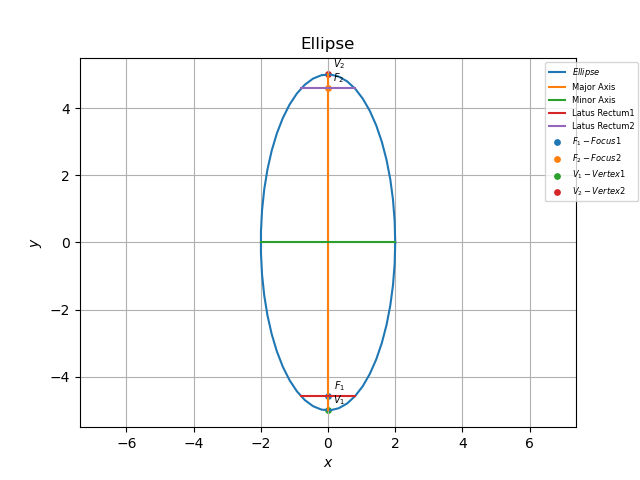
\includegraphics[width=\columnwidth]{chapters/11/11/3/2/figs/ellipse}
	\end{center}
\caption{}
\label{fig:chapters/11/11/3/2/Fig1}
\end{figure}

  \item $\frac{x^2}{16}+\frac{y^2}{9}=1$
\\
\solution
%\iffalse
\documentclass[12pt]{article}
\usepackage{graphicx}
\usepackage[none]{hyphenat}
\usepackage{graphicx}
\usepackage{listings}
\usepackage[english]{babel}
\usepackage{graphicx}
\usepackage{caption} 
\usepackage{booktabs}
\usepackage{array}
\usepackage{amssymb} % for \because
\usepackage{amsmath}   % for having text in math mode
\usepackage{extarrows} % for Row operations arrows
\usepackage{listings}
\lstset{
  frame=single,
  breaklines=true
}
\usepackage{hyperref}
  
%Following 2 lines were added to remove the blank page at the beginning
\usepackage{atbegshi}% http://ctan.org/pkg/atbegshi
\AtBeginDocument{\AtBeginShipoutNext{\AtBeginShipoutDiscard}}


%New macro definitions
\newcommand{\mydet}[1]{\ensuremath{\begin{vmatrix}#1\end{vmatrix}}}
\providecommand{\brak}[1]{\ensuremath{\left(#1\right)}}
\providecommand{\norm}[1]{\left\lVert#1\right\rVert}
\providecommand{\abs}[1]{\left\vert#1\right\vert}
\newcommand{\solution}{\noindent \textbf{Solution: }}
\newcommand{\myvec}[1]{\ensuremath{\begin{pmatrix}#1\end{pmatrix}}}
\let\vec\mathbf


\begin{document}

\begin{center}
\title{\textbf{Conic Sections - Ellipse}}
\date{\vspace{-5ex}} %Not to print date automatically
\maketitle
\end{center}
\setcounter{page}{1}

\section{11$^{th}$ Maths - Chapter 11}
This is Problem-3 from Exercise 11.3
\begin{enumerate}
\item Find the coordinates of the focii, the vertices, the length of major and minor axes, the eccentricity and the length of the latus rectum of an ellipse whose equation is given by $\frac{x^2}{16}+\frac{y^2}{9}=1$.

\solution
\fi
The given equation of ellipse can be rearranged as 
\begin{align}
 9x^2+16y^2-144=0\label{eq:chapters/11/11/3/3/eq1}
\end{align}
The above equation can be equated to the general equation of conic sections
\begin{align}
 g\brak{\vec{x}}=\vec{x}^\top \vec{V} \vec{x} + 2\vec{u}^\top \vec{x} + f = 0\label{eq:chapters/11/11/3/3/eq2}
\end{align}
From \eqref{eq:chapters/11/11/3/3/eq1} and \eqref{eq:chapters/11/11/3/3/eq2}
\begin{align}
 \vec{V} &= \myvec{9&0\\0&16}\label{eq:chapters/11/11/3/3/eq3}\\
 \vec{u} &= \vec{0}\\
 f &= -144
\end{align}
From \eqref{eq:chapters/11/11/3/3/eq3} the eigen values $\lambda_1 \text{ and } \lambda_2$ are given as
\begin{align}
 \lambda_1 &= 9\\
 \lambda_2 &= 16
\end{align}
\begin{enumerate}
\item The eccentricity of the ellipse is given as
\begin{align}
 e &= \sqrt{1 - \frac{\lambda_2}{\lambda_1}} \\
          &= \sqrt{1-\frac{9}{16}}\\
   &= \frac{\sqrt{7}}{4}
\end{align}
\item Finding the coordinates of Focii
\begin{align}
 \vec{F} &= \pm e\sqrt{\frac{\abs{f_0}}{\lambda_2\brak{1-e^2}}}\Vec{e_1}\\
\text{Where }f_0 &=-f\\
 \vec{F} &= \pm\sqrt{7}\myvec{1\\0}\\
	&= \pm\myvec{\sqrt{7}\\0}
\end{align}
\item The length of the major axis is given by
\begin{align}
 &2\sqrt{\abs{\frac{f_0}{\lambda_1}}}\\
        &2\sqrt{\abs{\frac{144}{9}}}= 8
\end{align}
\item The length of minor axis is given by
\begin{align}
 &2\sqrt{\abs{\frac{f_0}{\lambda_2}}}\\
        &2\sqrt{\abs{\frac{144}{16}}}= 6
\end{align}
\item The vertices of the ellipse are given by
\begin{align}
 \pm \myvec{0\\\sqrt{\abs{\frac{f_0}{\lambda_2}}}}= \pm \myvec{0\\4}
\end{align}
\item The length of latus rectum is given as
\begin{align}
 &2\frac{\sqrt{\abs{f_0 \lambda_1}}}{\lambda_2} \\
 &= 2\frac{\sqrt{\abs{144\brak{9}}}}{16}\\
 &= \frac{9}{2}
\end{align}
\begin{figure}[!h]
	\begin{center}
		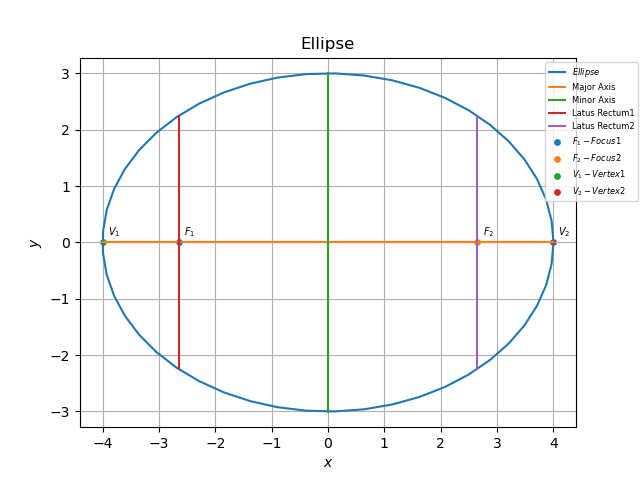
\includegraphics[width=\columnwidth]{chapters/11/11/3/3/figs/conic.png}
	\end{center}
\caption{}
\label{fig:chapters/11/11/3/3/Fig1}
\end{figure}
\end{enumerate}

  \item $\frac{x^2}{25}+\frac{y^2}{100}=1$
  \item $\frac{x^2}{49}+\frac{y^2}{36}=1$
  \item $\frac{x^2}{100}+\frac{y^2}{400}=1$
  \item $36x^2+4y^2=144$
  \item $16x^2+y^2=16$
  \item $4x^2+9y^2=36$
	\item Find the coordinates of the focii, the vertices, the eccentricity and the length of the latus rectum of a hyperbola whose equation is given by $\frac{x^2}{16}-\frac{y^2}{9} = 1$. \\ 
		\solution
		%See 
\tabref{tab:std-conic-params-sol}
and
\figref{fig:11/11/4/1Fig1}.
\begin{figure}[!h]
	\begin{center}
		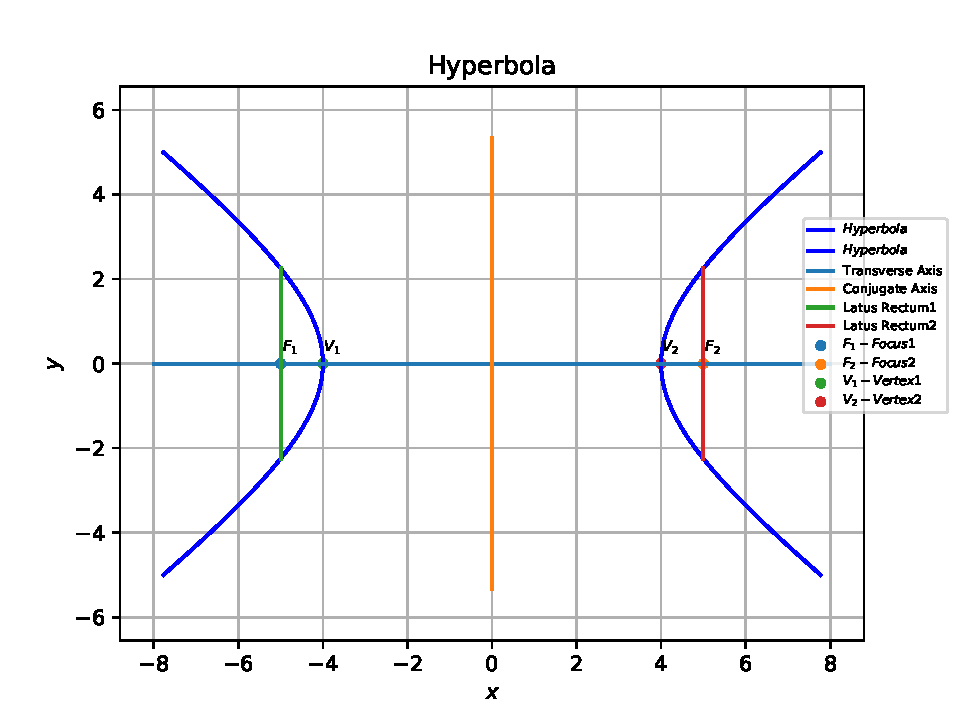
\includegraphics[width=\columnwidth]{chapters/11/11/4/1/figs/problem1.pdf}
	\end{center}
\caption{}
\label{fig:11/11/4/1Fig1}
\end{figure}

	\item Find the coordinates of the focii, the vertices, the eccentricity and the length of the latus rectum of a hyperbola whose equation is given by $\frac{y^2}{9}-\frac{x^2}{27}=1$.
		\\
		\solution
		\\
		%See \tabref{tab:rot-conic-params-sol}
and 
\figref{fig:chapters/11/11/4/2/Fig1}.
\begin{figure}[H]
	\begin{center} 
	    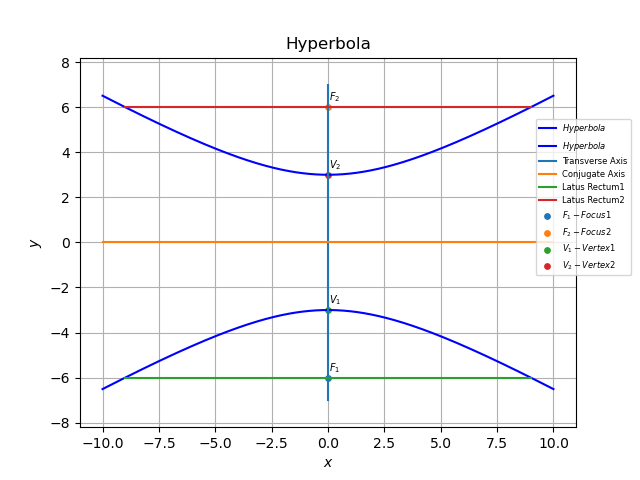
\includegraphics[width=0.75\columnwidth]{chapters/11/11/4/2/figs/hyperbola}
	\end{center}
\caption{}
\label{fig:chapters/11/11/4/2/Fig1}
\end{figure}




	\item Find the coordinates of the foci and the vertices, the eccentricity and the length of the latus rectum of the hyperbolas, whose equation is given by $5{y^2}-9{x^2}=36$.
		\\
		\solution
		\\
		%\iffalse
\documentclass[journal,12pt,twocolumn]{IEEEtran}
\usepackage{setspace}
\usepackage{gensymb}
\usepackage{xcolor}
\usepackage{caption}
\singlespacing
\usepackage{siunitx}
\usepackage[cmex10]{amsmath}
\usepackage{mathtools}
\usepackage{hyperref}
\usepackage{amsthm}
\usepackage{mathrsfs}
\usepackage{txfonts}
\usepackage{stfloats}
\usepackage{cite}
\usepackage{cases}
\usepackage{subfig}
\usepackage{longtable}
\usepackage{multirow}
\usepackage{enumitem}
\usepackage{bm}
\usepackage{mathtools}
\usepackage{listings}
\usepackage{tikz}
\usetikzlibrary{shapes,arrows,positioning}
\usepackage{circuitikz}
\renewcommand{\vec}[1]{\boldsymbol{\mathbf{#1}}}
\DeclareMathOperator*{\Res}{Res}
\renewcommand\thesection{\arabic{section}}
\renewcommand\thesubsection{\thesection.\arabic{subsection}}
\renewcommand\thesubsubsection{\thesubsection.\arabic{subsubsection}}

\renewcommand\thesectiondis{\arabic{section}}
\renewcommand\thesubsectiondis{\thesectiondis.\arabic{subsection}}
\renewcommand\thesubsubsectiondis{\thesubsectiondis.\arabic{subsubsection}}
\hyphenation{op-tical net-works semi-conduc-tor}

\lstset{
language=Python,
frame=single, 
breaklines=true,
columns=fullflexible
}
\begin{document}
\theoremstyle{definition}
\newtheorem{theorem}{Theorem}[section]
\newtheorem{problem}{Problem}
\newtheorem{proposition}{Proposition}[section]
\newtheorem{lemma}{Lemma}[section]
\newtheorem{corollary}[theorem]{Corollary}
\newtheorem{example}{Example}[section]
\newtheorem{definition}{Definition}[section]
\newcommand{\BEQA}{\begin{eqnarray}}
        \newcommand{\EEQA}{\end{eqnarray}}
\newcommand{\define}{\stackrel{\triangle}{=}}
\newcommand{\myvec}[1]{\ensuremath{\begin{pmatrix}#1\end{pmatrix}}}
\newcommand{\mydet}[1]{\ensuremath{\begin{vmatrix}#1\end{vmatrix}}}
\bibliographystyle{IEEEtran}
\providecommand{\nCr}[2]{\,^{#1}C_{#2}} % nCr
\providecommand{\nPr}[2]{\,^{#1}P_{#2}} % nPr
\providecommand{\mbf}{\mathbf}
\providecommand{\pr}[1]{\ensuremath{\Pr\left(#1\right)}}
\providecommand{\qfunc}[1]{\ensuremath{Q\left(#1\right)}}
\providecommand{\sbrak}[1]{\ensuremath{{}\left[#1\right]}}
\providecommand{\lsbrak}[1]{\ensuremath{{}\left[#1\right.}}
\providecommand{\rsbrak}[1]{\ensuremath{{}\left.#1\right]}}
\providecommand{\brak}[1]{\ensuremath{\left(#1\right)}}
\providecommand{\lbrak}[1]{\ensuremath{\left(#1\right.}}
\providecommand{\rbrak}[1]{\ensuremath{\left.#1\right)}}
\providecommand{\cbrak}[1]{\ensuremath{\left\{#1\right\}}}
\providecommand{\lcbrak}[1]{\ensuremath{\left\{#1\right.}}
\providecommand{\rcbrak}[1]{\ensuremath{\left.#1\right\}}}
\theoremstyle{remark}
\newtheorem{rem}{Remark}
\newcommand{\sgn}{\mathop{\mathrm{sgn}}}
\newcommand{\rect}{\mathop{\mathrm{rect}}}
\newcommand{\sinc}{\mathop{\mathrm{sinc}}}
\providecommand{\abs}[1]{\left\vert#1\right\vert}
\providecommand{\res}[1]{\Res\displaylimits_{#1}}
\providecommand{\norm}[1]{\lVert#1\rVert}
\providecommand{\mtx}[1]{\mathbf{#1}}
\providecommand{\mean}[1]{E\left[ #1 \right]}
\providecommand{\fourier}{\overset{\mathcal{F}}{ \rightleftharpoons}}
\providecommand{\ztrans}{\overset{\mathcal{Z}}{ \rightleftharpoons}}
\providecommand{\system}[1]{\overset{\mathcal{#1}}{ \longleftrightarrow}}
\newcommand{\solution}{\noindent \textbf{Solution: }}
\providecommand{\dec}[2]{\ensuremath{\overset{#1}{\underset{#2}{\gtrless}}}}
\let\StandardTheFigure\thefigure
\def\putbox#1#2#3{\makebox[0in][l]{\makebox[#1][l]{}\raisebox{\baselineskip}[0in][0in]{\raisebox{#2}[0in][0in]{#3}}}}
\def\rightbox#1{\makebox[0in][r]{#1}}
\def\centbox#1{\makebox[0in]{#1}}
\def\topbox#1{\raisebox{-\baselineskip}[0in][0in]{#1}}
\def\midbox#1{\raisebox{-0.5\baselineskip}[0in][0in]{#1}}

\vspace{3cm}
\title{11.11.4.5}
\author{Lokesh Surana}
\maketitle
\section*{Class 11, Chapter 11, Exercise 4.5}
\fi
The equation of the hyperbola can be rearranged as
\begin{align}
	\label{eq:chapters/11/11/4/5/1}
	-x^2 + \frac{5}{9}y^2 -4 = 0
\end{align}
The above equation can be equaded to the generic equation of conic sections
\begin{align}
	\label{eq:chapters/11/11/4/5/2}
	g\brak{\vec{x}}=\vec{x}^\top \vec{V} \vec{x} + 2\vec{u}^\top \vec{x} + f = 0
\end{align}
Comparing coefficients of both equations \eqref{eq:chapters/11/11/4/5/1} and \eqref{eq:chapters/11/11/4/5/2}
\begin{align}
	\label{3}
	\vec{V} &= \myvec{-1&0\\0&\frac{5}{9}}\\
	\vec{u} &= \vec{0}\\
	f &= -4
\end{align}

From equation \eqref{3}, since $\vec{V}$ is already diagonalized, the eigen values $\lambda_1 \text{ and } \lambda_2$ are given as
\begin{align}
	\lambda_1 &= -1\\
	\lambda_2 &= \frac{5}{9}
\end{align}
\begin{enumerate}
\item The eccentricity of the hyperbola is given as
\begin{align}
	e &= \sqrt{1 - \frac{\lambda_2}{\lambda_1}} = \sqrt{1+\frac{5}{9}}\\
	  &= \frac{\sqrt{14}}{3}
\end{align}
\item For the standard hyperbola, the coordinates of Focii are given as
\begin{align}
	\label{eq:chapters/11/11/4/5/4}
	\vec{F} = \pm \frac{\brak{\frac{1}{e\sqrt{1-e^2}}}\brak{e^2}\sqrt{\frac{\lambda_1}{f_0}}}{\frac{\lambda_1}{f_0}} \vec{e}_2
\end{align}
where
\begin{align}
	f_0 &= -f\\
	\eqref{eq:chapters/11/11/4/5/4} \implies &= \pm \frac{\brak{\frac{1}{\frac{\sqrt{14}}{3}\sqrt{1-\frac{14}{9}}}}\brak{\frac{14}{9}}\sqrt{\frac{-1}{4}}}{\frac{-1}{4}} \vec{e}_2\\
	&= \pm \myvec{0\\\frac{6}{2\sqrt{\frac{14}{5}}}}
\end{align}
\item The vertices of the hyperbola are given by
\begin{align}
	\pm \myvec{0\\\sqrt{\abs{\frac{f_0}{\lambda_2}}}}= \pm \myvec{0\\\frac{6}{\sqrt{5}}}
\end{align}
\item The length of latus rectum is given as
\begin{align}
	2\frac{\sqrt{\abs{f_0 \lambda_2}}}{\lambda_1} &= 2\frac{\sqrt{\abs{14\brak{\frac{5}{9}}}}}{-1}\\
	&= 4\frac{\sqrt{5}}{3}
\end{align}
as length cannot be negative.
\end{enumerate}

\begin{figure}[!h]
	\begin{center} 
	    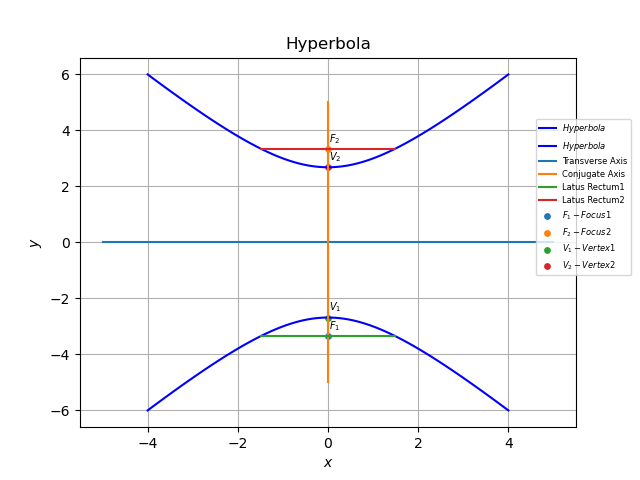
\includegraphics[width=\columnwidth]{chapters/11/11/4/5/figs/hyperbola.png}
	\end{center}
\caption{}
\label{fig:chapters/11/11/4/5/1}
\end{figure}


	\item Find the equation of the hyperbola whose foci is $\brak{0,\pm 8}$ and vertices $\brak{0,\pm 5}$.
\\
\solution
\end{enumerate}

Each of the Exercises, find the equation of the parabola, that satisfies the given conditions.

\begin{enumerate}[label=\thesubsection.\arabic*,ref=\thesubsection.\theenumi,resume*]
\item Focus(6,0); directrix x=-6 
\item Focus(0,-3); directrix y=3
\item Vertex(0,0); Focus(3,0)
\item Vertex(0,0); Focus(-2,0) 
\item Vertex(0,0) passing through(2,3) and axis is along x-axis
\item Vertex(0,0) passing through(5,2) symmetric with respect to y-axis
\item vertices $(\pm5,0),\text{foci} (\pm4,0)$
\item vertices $(\pm0,13),\text{foci} (0,\pm5)$
\item vertices $(\pm6,0),\text{foci} (\pm4,0)$
\item Ends of major axis $(\pm3,0),\text{ends of minor axis}(0,\pm2)$
\item  ends of major axis $(0,\pm \sqrt{5}),\text{ends of minor axis} (\pm1,0)$
\item $\text {length of major axis 26},\text{foci} (\pm5,0)$
\item $\text {length of minor axis 16},\text{foci} (0,\pm6)$
\item $\text {foci} (\pm3,0),a=4$
\item $\text {b=3,c=4},\text {centre at the origin} ;\text{foci on the x axis}$
\item $\text {centre at} (0,0),\text{major axis on the y-axis and passes through the points} \text {(3,2) and (1,6)}$.
\\
\solution
%%Since the major axis is along the $y$-axis,
\begin{align}
\vec{n} = \vec{e}_2
\end{align}
Thus,
\begin{align}
\vec{V} = \myvec{1&0\\0&1-e^2} \label{eq:chapters/11/11/3/19/5} 
\end{align}
Since
\begin{align}
\vec{c} = \vec{0}, \vec{u}=\vec{0}.
\label{eq:chapters/11/11/3/19/8}
\end{align}
    From \eqref{eq:conic_quad_form},
    \begin{align}
        \vec{P}^\top\vec{VP} + 2\vec{u}^\top\vec{P} + f &= 0 \label{eq:chapters/11/11/3/19/ep1} \\
        \vec{Q}^\top\vec{VQ} + 2\vec{u}^\top\vec{Q} + f &= 0 \label{eq:chapters/11/11/3/19/ep2}
    \end{align}
    yielding
\begin{align}
4e^2 - f = 13 \label{eq:chapters/11/11/3/19/10}
\\
36e^2 - f = 37 \label{eq:chapters/11/11/3/19/11}
\end{align}
which can be formulated as the matrix equation
\begin{align}
\myvec{4&-1\\36&-1}\myvec{e^2\\f} = \myvec{13\\37}
\label{eq:chapters/11/11/3/19/12}
\end{align}
The augmented matrix is given by,
\begin{align*}
\myvec{4&-1&\vline&13\\36&-1&\vline&37}
\xleftrightarrow[]{R_1\leftarrow-\frac{R_1}{8}} \myvec{4&0&\vline&3\\36&-1&\vline&37} 
\\
\xleftrightarrow[]{R_2\leftarrow R_2-9R_1}
\myvec{4&0&\vline&3\\0&-1&\vline&10} 
\xleftrightarrow[R_2\leftarrow -R_2]{R_1\leftarrow \frac{R_1}{4}}
\myvec{1&0&\vline&\frac{3}{4}\\0&1&\vline&-10}
\end{align*}
Thus,
\begin{align}
e^2 = \frac{3}{4},\ f = -10
\end{align}
and the equation of the conic is given by
\begin{align}
\vec{x}^\top\myvec{1&0\\0&\frac{1}{4}}\vec{x} - 10 = 0
\end{align}
See  
\figref{fig:chapters/11/11/3/19/1}.
\begin{figure}[ht]
\centering
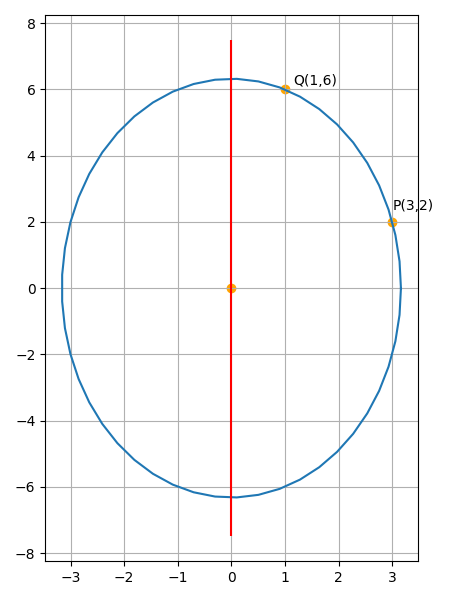
\includegraphics[width = \columnwidth]{chapters/11/11/3/19/figs/fig1.png}
\caption{Graph}
\label{fig:chapters/11/11/3/19/1}
\end{figure}

\item $\text{major axis on the x-axis and passes through the points (4,3) and (6,2)}$
\\
\solution
%%In this case, 
    \begin{align}
        \vec{n} = \myvec{1\\0}
    \end{align}
    Thus,
    \begin{align}
        \vec{V} = \myvec{1-e^2&0\\0&1} \label{eq:chapters/11/11/3/20/V-val} \\
    \end{align}
Since
\begin{align}
\vec{c} = \vec{0}, \vec{u}=\vec{0}.
\label{eq:chapters/11/11/3/20/8}
    \end{align}
    From \eqref{eq:conic_quad_form},
    \begin{align}
        \vec{P}^\top\vec{VP} + 2\vec{u}^\top\vec{P} + f &= 0 \label{eq:chapters/11/11/3/20/ep1} \\
        \vec{Q}^\top\vec{VQ} + 2\vec{u}^\top\vec{Q} + f &= 0 \label{eq:chapters/11/11/3/20/ep2}
    \end{align}
    yielding
    \begin{align}
        16e^2 - f = 25 \label{eq:chapters/11/11/3/20/e1}
	\\
        36e^2 - f = 40 \label{eq:chapters/11/11/3/20/e2}
    \end{align}
which can be formulated as the matrix equation
    \begin{align}
        \myvec{16&-1\\36&-1}\myvec{e^2\\f} = \myvec{25\\40}
        \label{eq:chapters/11/11/3/20/mtx-eqn}
    \end{align}
    and can be solved using the augmented matrix.
    \begin{align*}
        \myvec{16&-1&25\\36&-1&40} \xleftrightarrow[]{R_1\leftarrow R_1-R_2} \myvec{-20&0&-15\\36&-1&40} \\
                 \xleftrightarrow[]{\substack{R_1\leftarrow\frac{R_1}{-5}\\R_2\leftarrow -R_2}} \myvec{4&0&3\\-36&1&-40} 
                 \xleftrightarrow[]{R_2\leftarrow R_2+9R_1}\myvec{4&0&3\\0&1&-13} \\
                 \xleftrightarrow[]{R_1\leftarrow\frac{R_1}{4}}\myvec{1&0&\frac{3}{4}\\0&1&-13}
    \end{align*}
    Thus,
    \begin{align}
        e^2 = \frac{3}{4},\ f = -13
    \end{align}
    and the equation of the conic is given by
    \begin{align}
        \vec{x}^\top\myvec{\frac{1}{4}&0\\0&1}\vec{x} - 13 = 0
    \end{align}
    See \figref{fig:chapters/11/11/3/20/ellipse}.
    \begin{figure}[H]
        \centering
        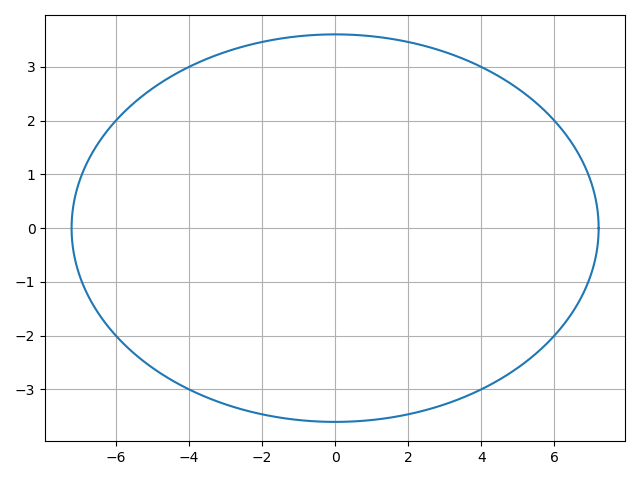
\includegraphics[width=0.75\columnwidth]{chapters/11/11/3/20/figs/ellipse.png}
        \caption{Locus of the required ellipse.}
        \label{fig:chapters/11/11/3/20/ellipse}
    \end{figure}

\item Find the equations of hyperbola having Vertices $\myvec{0\\\pm 3}$ and Foci $\myvec{0\\\pm5}$
	\\
\solution
		%\iffalse
\documentclass[journal,12pt,twocolumn]{IEEEtran}
%
\usepackage{setspace}
\usepackage{gensymb}
%\doublespacing
\singlespacing

%\usepackage{graphicx}
%\usepackage{amssymb}
%\usepackage{relsize}
\usepackage[cmex10]{amsmath}
%\usepackage{amsthm}
%\interdisplaylinepenalty=2500
%\savesymbol{iint}
%\usepackage{txfonts}
%\restoresymbol{TXF}{iint}
%\usepackage{wasysym}
\usepackage{amsthm}
%\usepackage{iithtlc}
\usepackage{mathrsfs}
\usepackage{txfonts}
\usepackage{stfloats}
\usepackage{bm}
\usepackage{cite}
\usepackage{cases}
\usepackage{subfig}
%\usepackage{xtab}
\usepackage{longtable}
\usepackage{multirow}
%\usepackage{algorithm}
%\usepackage{algpseudocode}
\usepackage{enumitem}
\usepackage{mathtools}
\usepackage{steinmetz}
\usepackage{tikz}
\usepackage{circuitikz}
\usepackage{verbatim}
\usepackage{tfrupee}
\usepackage[breaklinks=true]{hyperref}
%\usepackage{stmaryrd}
\usepackage{tkz-euclide} % loads  TikZ and tkz-base
%\usetkzobj{all}
\usetikzlibrary{calc,math}
\usepackage{listings}
    \usepackage{color}                                            %%
    \usepackage{array}                                            %%
    \usepackage{longtable}                                        %%
    \usepackage{calc}                                             %%
    \usepackage{multirow}                                         %%
    \usepackage{hhline}                                           %%
    \usepackage{ifthen}                                           %%
  %optionally (for landscape tables embedded in another document): %%
    \usepackage{lscape}     
\usepackage{multicol}
\usepackage{chngcntr}
%\usepackage{enumerate}

%\usepackage{wasysym}
%\newcounter{MYtempeqncnt}
\DeclareMathOperator*{\Res}{Res}
%\renewcommand{\baselinestretch}{2}
\renewcommand\thesection{\arabic{section}}
\renewcommand\thesubsection{\thesection.\arabic{subsection}}
\renewcommand\thesubsubsection{\thesubsection.\arabic{subsubsection}}

\renewcommand\thesectiondis{\arabic{section}}
\renewcommand\thesubsectiondis{\thesectiondis.\arabic{subsection}}
\renewcommand\thesubsubsectiondis{\thesubsectiondis.\arabic{subsubsection}}

% correct bad hyphenation here
\hyphenation{op-tical net-works semi-conduc-tor}
\def\inputGnumericTable{}                                 %%

\lstset{
%language=C,
frame=single, 
breaklines=true,
columns=fullflexible
}
%\lstset{
%language=tex,
%frame=single, 
%breaklines=true
%}

\begin{document}
%


\newtheorem{theorem}{Theorem}[section]
\newtheorem{problem}{Problem}
\newtheorem{proposition}{Proposition}[section]
\newtheorem{lemma}{Lemma}[section]
\newtheorem{corollary}[theorem]{Corollary}
\newtheorem{example}{Example}[section]
\newtheorem{definition}[problem]{Definition}
%\newtheorem{thm}{Theorem}[section] 
%\newtheorem{defn}[thm]{Definition}
%\newtheorem{algorithm}{Algorithm}[section]
%\newtheorem{cor}{Corollary}
\newcommand{\BEQA}{\begin{eqnarray}}
\newcommand{\EEQA}{\end{eqnarray}}
\newcommand{\define}{\stackrel{\triangle}{=}}

\bibliographystyle{IEEEtran}
%\bibliographystyle{ieeetr}


\providecommand{\mbf}{\mathbf}
\providecommand{\pr}[1]{\ensuremath{\Pr\left(#1\right)}}
\providecommand{\qfunc}[1]{\ensuremath{Q\left(#1\right)}}
\providecommand{\sbrak}[1]{\ensuremath{{}\left[#1\right]}}
\providecommand{\lsbrak}[1]{\ensuremath{{}\left[#1\right.}}
\providecommand{\rsbrak}[1]{\ensuremath{{}\left.#1\right]}}
\providecommand{\brak}[1]{\ensuremath{\left(#1\right)}}
\providecommand{\lbrak}[1]{\ensuremath{\left(#1\right.}}
\providecommand{\rbrak}[1]{\ensuremath{\left.#1\right)}}
\providecommand{\cbrak}[1]{\ensuremath{\left\{#1\right\}}}
\providecommand{\lcbrak}[1]{\ensuremath{\left\{#1\right.}}
\providecommand{\rcbrak}[1]{\ensuremath{\left.#1\right\}}}
\theoremstyle{remark}
\newtheorem{rem}{Remark}
\newcommand{\sgn}{\mathop{\mathrm{sgn}}}
\providecommand{\abs}[1]{\left\vert#1\right\vert}
\providecommand{\res}[1]{\Res\displaylimits_{#1}} 
\providecommand{\norm}[1]{\left\lVert#1\right\rVert}
%\providecommand{\norm}[1]{\lVert#1\rVert}
\providecommand{\mtx}[1]{\mathbf{#1}}
\providecommand{\mean}[1]{E\left[ #1 \right]}
\providecommand{\fourier}{\overset{\mathcal{F}}{ \rightleftharpoons}}
%\providecommand{\hilbert}{\overset{\mathcal{H}}{ \rightleftharpoons}}
\providecommand{\system}{\overset{\mathcal{H}}{ \longleftrightarrow}}
	%\newcommand{\solution}[2]{\textbf{Solution:}{#1}}
\newcommand{\solution}{\noindent \textbf{Solution: }}
\newcommand{\cosec}{\,\text{cosec}\,}
\providecommand{\dec}[2]{\ensuremath{\overset{#1}{\underset{#2}{\gtrless}}}}
\newcommand{\myvec}[1]{\ensuremath{\begin{pmatrix}#1\end{pmatrix}}}
\newcommand{\mydet}[1]{\ensuremath{\begin{vmatrix}#1\end{vmatrix}}}
%\numberwithin{equation}{section}
\numberwithin{equation}{subsection}
%\numberwithin{problem}{section}
%\numberwithin{definition}{section}
\makeatletter
\@addtoreset{figure}{problem}
\makeatother

\let\StandardTheFigure\thefigure
\let\vec\mathbf
%\renewcommand{\thefigure}{\theproblem.\arabic{figure}}
\renewcommand{\thefigure}{\theproblem}
%\setlist[enumerate,1]{before=\renewcommand\theequation{\theenumi.\arabic{equation}}
%\counterwithin{equation}{enumi}


%\renewcommand{\theequation}{\arabic{subsection}.\arabic{equation}}

\def\putbox#1#2#3{\makebox[0in][l]{\makebox[#1][l]{}\raisebox{\baselineskip}[0in][0in]{\raisebox{#2}[0in][0in]{#3}}}}
     \def\rightbox#1{\makebox[0in][r]{#1}}
     \def\centbox#1{\makebox[0in]{#1}}
     \def\topbox#1{\raisebox{-\baselineskip}[0in][0in]{#1}}
     \def\midbox#1{\raisebox{-0.5\baselineskip}[0in][0in]{#1}}

\vspace{3cm}


\title{Que: 11.11.4.9}
\author{Nikam Pratik Balasaheb (EE21BTECH11037)}





% make the title area
\maketitle

\newpage

%\tableofcontents

\bigskip

\renewcommand{\thefigure}{\theenumi}
\renewcommand{\thetable}{\theenumi}
%\renewcommand{\theequation}{\theenumi}

\section{Problem}

\section{Solution}
\fi

\begin{enumerate}

	\item Transverse axis:
Line joining two foci
\begin{align}
	\vec{m} &= \vec{F}_1 - \vec{F}_2\\
	&= \myvec{0 \\ 10}\\
	\myvec{1&0}\brak{\vec{x} -\vec{F}_1} &= 0\\
	\myvec{1& 0}\vec{x} &= 0
\end{align}

\item Center of hyperbola, $\vec{O}$ is given by:
\begin{align}
	\vec{O} &= \frac{\vec{F}_1 + \vec{F}_2}{2}\\
	\vec{O} &= \myvec{0\\0}
\end{align}

\item Normal vector of directrix
	\begin{align}
		\vec{n} &= \text{direction vector of transverse axis}\\
			&= \myvec{0 \\1}
	\end{align}
%
\begin{align}
	\vec{V} &= \norm{\vec{n}}^2\vec{I} - e^2\vec{n}\vec{n}^{\top}\\
		&= \myvec{1 & 0 \\ 0 & 1} - e^2\myvec{ 0 & 0 \\ 0 & 1}\\
		&= \myvec{1 &0\\ 0 & 1-e^2}
\end{align}
%
\begin{align}
	\vec{u} &= ce^2\vec{n} -\norm{\vec{n}}^2\vec{F}\\
		&= \myvec{0\\ ce^2 - 5}
\end{align}
%
\begin{align}
	f &= \norm{\vec{n}}^2\norm{\vec{F}}^2 - c^2e^2\\
	  &= 25 - c^2 e^2
\end{align}
%
Equation of the hyperbola
\begin{align}
	\vec{x}^{\top}\vec{V}\vec{x} +2\vec{u}^{\top}\vec{x}+f &= 0
\end{align}
%
Vertex lies on this curve,
\begin{align}
	\vec{v_1}^{\top}\vec{V}\vec{v_1} +2\vec{u}^{\top}\vec{v_1}+f &= 0\\
	9\brak{1-e^2} + 6 \brak{ce^2 -5} - c^2e^2 +25 &= 0\\
	4 -9e^2 +6ce^2 -c^2e^2 &= 0 \label{eq:chapters/11/11/4/9/1}
\end{align}
Also, the center is given by,
\begin{align}
	\vec{O} &= - \vec{V}^{-1} \vec{u}\\
	\myvec{0\\0} &= \myvec{0\\ \frac{ce^2-5}{1-e^2}}\\
	ce^2 &= 5
	\label{eq:chapters/11/11/4/9/2}
\end{align}
%
Solving \eqref{eq:chapters/11/11/4/9/1} and \eqref{eq:chapters/11/11/4/9/2},
\begin{align}
	c &= \frac{9}{5} \\
	e &= \frac{5}{3}
\end{align}
%
\begin{align}
	\vec{V} &= \myvec{1&0\\0& -\frac{16}{9}} \\
	\vec{u} &= \myvec{0\\0}\\
	f &= 16
\end{align}
%
Equation of the Hyperbola,
\begin{align}
	\vec{x}^{\top} \myvec{1&0\\ 0 & -\frac{16}{9}} \vec{x} +16 =0
\end{align}
%
\begin{table}[h!]
	\begin{center}
	%%%%%%%%%%%%%%%%%%%%%%%%%%%%%%%%%%%%%%%%%%%%%%%%%%%%%%%%%%%%%%%%%%%%%%
%%                                                                  %%
%%  This is a LaTeX2e table fragment exported from Gnumeric.        %%
%%                                                                  %%
%%%%%%%%%%%%%%%%%%%%%%%%%%%%%%%%%%%%%%%%%%%%%%%%%%%%%%%%%%%%%%%%%%%%%%

\begin{tabular}[]{|c|c|c|}
\hline
Parameter & Value & Description \\ \hline
$\vec{F}_1$	& $\myvec{0\\5}$ & Focus\\ \hline
$\vec{F}_2$	& $\myvec{0\\-5}$ & Focus\\ \hline
$\vec{v}_1$	& $\myvec{0\\3}$ & Vertex \\ \hline
$\vec{v}_2$ 	& $\myvec{0\\-3}$ & Vertex\\ \hline
\end{tabular}

\end{center}
\caption{}
\label{tab:chapters/11/11/4/9/}
\end{table}
%
\begin{figure}[h!]
  \centering
    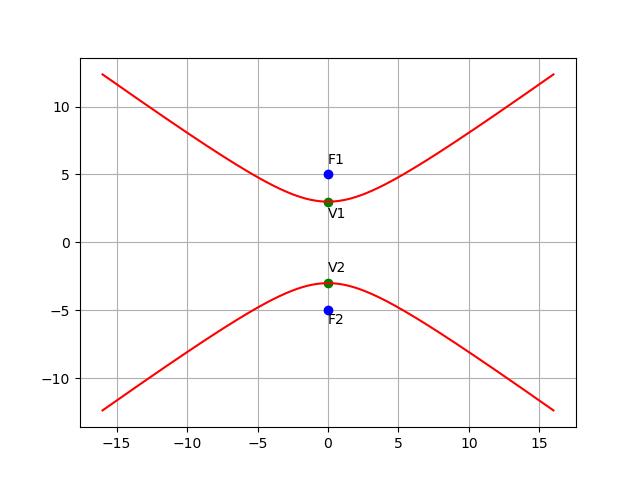
\includegraphics[width=\columnwidth]{chapters/11/11/4/9/figs/Figure_1.png}
    \caption{Figure 1}
    \label{fig:chapters/11/11/4/9/}
\end{figure}
%
\end{enumerate}




	%It is obvious that
	\begin{align}
		\vec{n} 
			= \vec{e}_2,
	\vec{c} =\vec{u}=\vec{0}.
\end{align}
Consequently,
%
\begin{align}
	\vec{V} &= \myvec{1 &0\\ 0 & 1-e^2}
	\\
	\vec{F} &= ce^2\vec{e}_2 \implies \norm{\vec{F}} = ce^2=8
\label{eq:chapters/11/11/4/8/F}
	\\
	f 
	  &= 64 - c^2 e^2
\label{eq:chapters/11/11/4/8/f}
\end{align}
%
Since the vertices are  on the conic,
\begin{align}
	\vec{v_1}^{\top}\vec{V}\vec{v_1} +2\vec{u}^{\top}\vec{v_1}+f &= 0\\
\implies 25\brak{1-e^2} + f &= 0\\
	 \label{eq:chapters/11/11/4/8/1}
\end{align}
Solving \eqref{eq:chapters/11/11/4/8/1},
\eqref{eq:chapters/11/11/4/8/F}
and
\eqref{eq:chapters/11/11/4/8/f},
\begin{align}
	c = \frac{9}{5},\ 
	e = \frac{5}{3},
\end{align}
%
yielding
\begin{align}
	\vec{V} = \myvec{1&0\\0& -\frac{16}{9}} ,\
	\vec{u} = \myvec{0\\0},\
	f = 16.
\end{align}
%
Thus, the desired equation of the hyperbola is
\begin{align}
	\vec{x}^{\top} \myvec{1&0\\ 0 & -\frac{16}{9}} \vec{x} +16 =0
\end{align}
%
\item We know the Focii is given as
\begin{align}
	\vec{F} &= \pm \frac{\brak{\frac{1}{e\sqrt{1-e^2}}}\brak{e^2}\sqrt{\frac{\lambda_1}{f_0}}}{\frac{\lambda_1}{f_0}}\vec{e}_2\\
	        &= \frac{\frac{e}{\sqrt{1-e^2}}}{\sqrt{\frac{\lambda_1}{f_0}}}\vec{e}_2
\end{align}
Substituting \eqref{eq:chapters/11/11/4/8/eq1} we get
\begin{align}
	\vec{F} &= 5e\vec{e}_2\\
	\myvec{0\\8} &= 5e\vec{e}_2\\
	\implies e &= \frac{8}{5}
\end{align}
\item Now we know the eccentricity is given as
\begin{align}
	e = \sqrt{1-\frac{\lambda_2}{\lambda_1}}\\
	\label{eq:chapters/11/11/4/8/eq2}
	\implies \frac{\lambda_2}{\lambda_1} = -\frac{39}{25}
\end{align}
\item Now we know from the standard equation
\begin{align}
	\label{eq:chapters/11/11/4/8/eq3}
	f = \norm{\vec{n}}^2 \norm{\vec{F}}^2 - c^2 e^2
\end{align}
Calculating $\vec{n} \text{ and } c$
\begin{align}
	\vec{n} &= \sqrt{\frac{\lambda_1}{f_0}}\vec{e}_2 = \frac{1}{5}\sqrt{\frac{\lambda_1}{\lambda_2}}\vec{e}_2\\
	        &= \frac{1}{\sqrt{-39}}\vec{e}_2\\
	c &= \frac{1}{e\sqrt{1-e^2}} = \frac{25}{8\sqrt{-39}}	
\end{align}
Now
\begin{align}
	\norm{\vec{n}}^2 &= -\frac{1}{39}\\
	\norm{\vec{F}}^2 &= 64
\end{align}
Substituting all the values in \eqref{eq:chapters/11/11/4/8/eq3} we get
\begin{align}
	f &= -\brak{\frac{1}{39}}\brak{64} + \brak{\frac{25}{8}}^2 \brak{\frac{1}{39}} \brak{\frac{64}{25}}\\
	  &= -1\\
	\label{eq:chapters/11/11/4/8/eq4}  
	f_0  &= -f = 1
\end{align}
substituting \eqref{eq:chapters/11/11/4/8/eq4} in \eqref{eq:chapters/11/11/4/8/eq1} we get
\begin{align}
	\label{eq:chapters/11/11/4/8/eq5}
	\lambda_2 = \frac{1}{25} 
\end{align}
Substituting \eqref{eq:chapters/11/11/4/8/eq5} in \eqref{eq:chapters/11/11/4/8/eq2} we get
\begin{align}
	\lambda_1 = -\frac{1}{39}
\end{align}
\end{enumerate}
Therefore the equation of the hyperbola is given as
\begin{align}
	g\brak{\vec{x}}=\vec{x}^\top \vec{V} \vec{x} + 2\vec{u}^\top \vec{x} + f = 0
\end{align}
where
\begin{align}
	\vec{V} &= \myvec{\lambda_1&0\\0&\lambda_2} = \myvec{-\frac{1}{39}&0\\0&\frac{1}{25}}\\
	\vec{u} &= \vec{0}\\
	f &= -1
\end{align}
See Fig. \ref{fig:chapters/11/11/4/8/Fig1}.
\begin{figure}[H]
	\begin{center} 
	    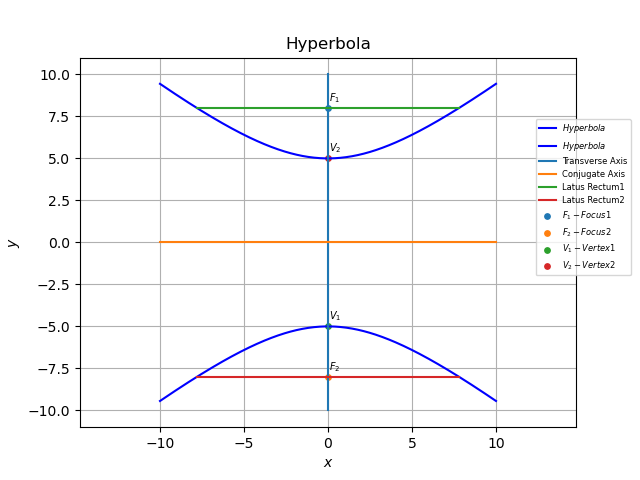
\includegraphics[width=0.75\columnwidth]{chapters/11/11/4/8/figs/hyperbola2}
	\end{center}
\caption{}
\label{fig:chapters/11/11/4/8/Fig1}
\end{figure}


\item Find the equation of the hyperbola that satisfies the conditions - Foci \brak{\pm 4, 0}, the latus rectum is of length 12.
\\
\solution
		%The given information is available in 
\tabref{tab:chapters/11/11/4/13/1}.
Since two foci are given, the conic cannot be a parabola.
The equation of the conic with focus $\vec{F}$, directrix $\vec{n}^\top\vec{x} = c$ and eccentricity $e$ is given by
\begin{align}
\vec{V} &\triangleq \norm{\vec{n}}^2\vec{I} - e^2\vec{n}\vec{n}^\top \label{eq:chapters/11/11/4/13/2} \\
\vec{u} &\triangleq ce^2\vec{n} - \norm{\vec{n}}^2\vec{F} \label{eq:chapters/11/11/4/13/3} \\
f &\triangleq \norm{\vec{n}}^2\norm{\vec{F}}^2 - c^2e^2 \label{eq:chapters/11/11/4/13/4}
\end{align}
also
\begin{align}
f_0 &= \vec{u}^\top\vec{V}^{-1}\vec{u} - f\\
l &= 2\frac{\sqrt{\abs{f_0\lambda_2}}}{\lambda_1}
\end{align}

\begin{enumerate}
\item The direction vector of $F_1F_2$ is the normal vector of the directrix.  Hence, 
\begin{align}
\vec{n} = \vec{F_1} - \vec{F_2}
	\equiv \vec{e}_1
\end{align}
Substituting in 
  \eqref{eq:conic_quad_form_v},
\eqref{eq:conic_quad_form_u}
and
\eqref{eq:conic_quad_form_f},
\begin{align}
	\vec{V} &= \myvec{1-e^2&0\\0&1} \label{eq:chapters/11/11/4/13/6} 
	\\
	\vec{u} &= ce^2\vec{e}_1-\vec{F}
\label{eq:chapters/11/11/4/13/6/u} 
	\\
	f&=16-c^2e^2
\label{eq:chapters/11/11/4/13/6/f} 
\end{align}
\item From
\eqref{eq:chapters/11/11/4/13/6},
\begin{align}
\lambda_1 &= 1-e^2,\
\lambda_2 = 1
\label{eq:chapters/11/11/4/13/12}
\end{align}
which upon substituting
in
			\eqref{eq:latus-ellipse}, along with the value of the latus rectum 
from \tabref{tab:chapters/11/11/4/13/1}
		\begin{align}
	6\brak{1-e^2} = \sqrt{\abs{f}}
\label{eq:chapters/11/11/4/13/12/f}
\end{align}
\item  The centre of the conic is given by
\begin{align}
\vec{c} = \frac{\vec{F_1} + \vec{F_2}}{2}
= \vec{0}
\label{eq:chapters/11/11/4/13/5}
\end{align}
From \eqref{eq:chapters/11/11/4/13/6}, it is obvious that  
$\vec{V}$ is invertible.  Hence,  
from \eqref{eq:chapters/11/11/4/13/5}
and 
\eqref{eq:conic_parmas_c_def},
\begin{align}
\vec{u} = \vec{0}
	\label{eq:chapters/11/11/4/13/7/u}
\end{align}
Substituting the above in \eqref{eq:chapters/11/11/4/13/6/u}, 
\begin{align}
\vec{F} = ce^2\vec{e}_1 
\implies 
	\norm{\vec{F}} = 4 = ce^2
	\label{eq:chapters/11/11/4/13/7}
\end{align}
\item 
	From 
      \eqref{eq:f0}, 
	\eqref{eq:chapters/11/11/4/13/7/u}
and
\eqref{eq:chapters/11/11/4/13/6/f},
		\begin{align}
	36\brak{1-e^2}^2 = 16-c^2e^2
\label{eq:chapters/11/11/4/13/12/ec}
\end{align}
From
	\eqref{eq:chapters/11/11/4/13/7}
	and
\eqref{eq:chapters/11/11/4/13/12/ec}
\begin{align}
\frac{4}{e\sqrt{e^2-1}} &= 6
\\
\implies 9e^2\brak{e^2-1} &= 4\\
\implies 9e^4-9e^2-4 &= 0
\\
	\text{or, }\brak{3e^2-4}
	\brak{12e^2+1} &=0
\label{eq:chapters/11/11/4/13/14}
\end{align}
yielding
\begin{align}
e = \frac{4}{3}
\end{align}
as the only viable solution.
\end{enumerate}
The equation of the conic is then obtained as
\begin{align}
\vec{x}^\top\myvec{-\frac{1}{3}&0\\0&1}\vec{x} +4 = 0
\end{align}
See \figref{fig:chapters/11/11/4/13/1}.
\begin{figure}[ht]
\centering
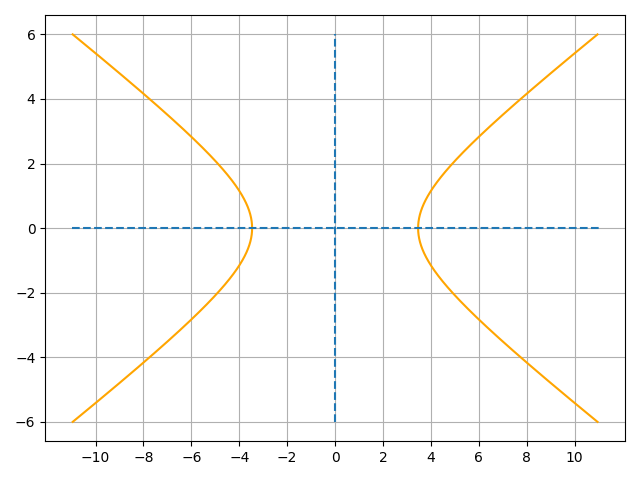
\includegraphics[width = \columnwidth]{chapters/11/11/4/13/figs/fig1.png}
\caption{}
\label{fig:chapters/11/11/4/13/1}
\end{figure}
\begin{table}[h]
\centering
%%%%%%%%%%%%%%%%%%%%%%%%%%%%%%%%%%%%%%%%%%%%%%%%%%%%%%%%%%%%%%%%%%%%%%
%%                                                                  %%
%%  This is a LaTeX2e table fragment exported from Gnumeric.        %%
%%                                                                  %%
%%%%%%%%%%%%%%%%%%%%%%%%%%%%%%%%%%%%%%%%%%%%%%%%%%%%%%%%%%%%%%%%%%%%%%

\begin{center}
\begin{tabular}{|c|c|c|}
\hline
\textbf{Parameter}& \textbf{Description} &\textbf{Value}\\ \hline
$\vec{F_1}$		 &	Focus 1 of hyperbola&$\myvec{4\\0}$\\ \hline
$\vec{F_2}$		 &	Focus 2 of hyperbola&$\myvec{-4\\0}$\\ \hline
$l$		 &  Length of latus rectum&12 \\ \hline
\end{tabular}
\end{center}

\caption{}
\label{tab:chapters/11/11/4/13/1}
\end{table}

    \item Find the equation of the hyperbola whose eccentricity is $e = \frac{4}{3}$
    and whose vertices are
    \begin{align}
        \vec{P_1} = \myvec{7\\0},\ \vec{P_2} = \myvec{-7\\0}
        \label{eq:chapters/11/11/4/14/vert}
    \end{align}
\\
\solution
		%    The major axis of a conic is the chord which passes through the vertices of the conic.
    The direction vector of the major axis in this case is
    \begin{align}
        \vec{P}_2-\vec{P}_1 \equiv \vec{e}_1 = \vec{n}
\label{eq:chapters/11/11/4/13/6/n} 
    \end{align}
    which is the normal vector for the directrix.
    Since $e > 1$, the conic is a hyperbola.
Substituting  
\eqref{eq:chapters/11/11/4/13/6/n} 
in
  \eqref{eq:conic_quad_form_v},
\eqref{eq:conic_quad_form_u}
and
\eqref{eq:conic_quad_form_f},
\begin{align}
	\vec{V} &= \myvec{1-e^2&0\\0&1} = \myvec{-\frac{7}{9}&0\\0&1} \label{eq:chapters/11/11/4/14/6} 
	\\
	\vec{u} &= ce^2\vec{e}_1-\vec{F}
\label{eq:chapters/11/11/4/14/6/u} 
	\\
	f&=16-c^2e^2
\label{eq:chapters/11/11/4/14/6/f} 
\end{align}
    Thus,
    \begin{align}
        \vec{V} = \myvec{1-e^2&0\\0&1} \label{eq:chapters/11/11/4/14/V-val} \\
	    \vec{u} = ce^2\vec{e}_1 - \vec{F} \label{eq:chapters/11/11/4/14/u-val} \\
        f = \norm{\vec{F}}^2 - c^2e^2 \label{eq:chapters/11/11/4/14/f-val}
    \end{align}
    The centre of the hyperbola is 
\begin{align}
	\vec{c} = \frac{\vec{P}_1+\vec{P}_2}{2} = \vec{0} = \vec{u}
\end{align}
from \eqref{eq:conic_parmas_c_def}.      Substituting $\vec{P}_1$ and $\vec{P}_2$ in 
    \eqref{eq:conic_quad_form},
    \begin{align}
        \vec{P}_1^\top\vec{VP}_1 + 2\vec{u}^\top\vec{P}_1 + f &= 0 \label{eq:chapters/11/11/4/14/ep1} \\
        \vec{P}_2^\top\vec{VP}_2 + 2\vec{u}^\top\vec{P}_2 + f &= 0 \label{eq:chapters/11/11/4/14/ep2}
	\\
	    \implies f = \vec{P}_1^\top\vec{VP}_1  = 49\brak{e^2-1}&=\frac{343}{9}
    \end{align}
    upon adding 
    \eqref{eq:chapters/11/11/4/14/ep2} and \eqref{eq:chapters/11/11/4/14/ep1}
    and simplifying.
    Therefore, the equation of the conic is
    \begin{align}
        \vec{x}^\top\myvec{-\frac{7}{9}&0\\0&1}\vec{x} + \frac{343}{9} = 0
    \end{align}
See \figref{fig:chapters/11/11/4/14/hyperbola}.
    \begin{figure}[!ht]
        \centering
        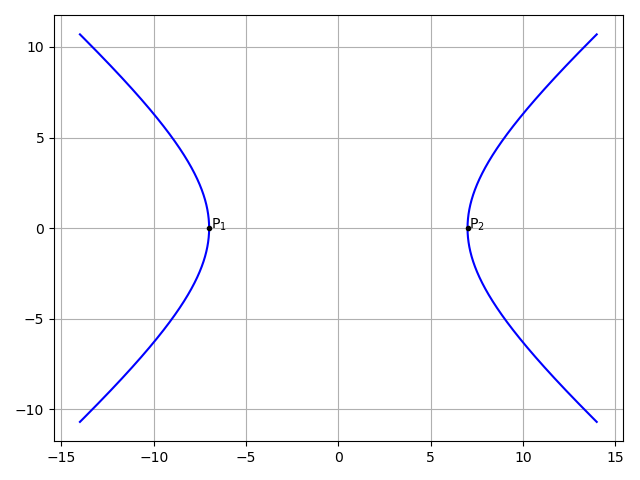
\includegraphics[width=\columnwidth]{chapters/11/11/4/14/figs/hyperbola.png}
        \caption{}
        \label{fig:chapters/11/11/4/14/hyperbola}
    \end{figure}

\item If the focus of a parabola is (0,-3) and its directrix is y=3, then its equation is
\begin{enumerate}
\item $x^2=-12y$
\item $x^2=12y$
\item $y^2=-12x$
\item $y^2=12x$
\end{enumerate}
\item If the parabola $y^2=4ax$ passes through the point (3,2), then the length of its latus rectum is
\begin{enumerate}
\item 2$\pm$3
\item 4$\pm$4
\item 1$\pm$3
\item 4
\end{enumerate}
\item If the vertex of the parabola is the point (-3,0) and the directrix is the line x+5=0, then its equation is
\begin{enumerate}
\item $y^2=8(x+3)$
\item $x^2=8(y+3)$
\item $y^2=-8(x+3)$
\item $y^2=8(x+5)$
\end{enumerate}
 \item Find the coordinates of a point on the parabla $y^2=8x$ whose focal distance is 4.
 \item Find the length of the line-segment joining the vertex of the parabola $y^2=4ax$ and a point on the parabola where the line - segment makes an angle 0 to the x-axis.
\item If the points (0,4) and (0,2) are respectively the vertex and focus of a parabola. then find the equation of the parabola
\end{enumerate}
Find the equation of each of the following parabolas
\begin{enumerate}[label=\thesection.\arabic*,ref=\thesection.\theenumi,resume*]
\item  Directrix x=0. focus ot (6,0)
\item  vertex  ot (0,4), focus at (0,2)
\item  Focus at (-1,2), directrix x-2y+3=0
\end{enumerate}
Fill in the Blanks
\begin{enumerate}[label=\thesection.\arabic*,ref=\thesection.\theenumi,resume*]
\item The equation of the parabola having focus at (-1,-2) and the directrix x-2y+3=0 is \makebox[1cm]{\hrulefill}   
\item show that the set of all points such that the difference of their distances from (4,0) and (-4,0) is always equal to 2 represent a hyperbola .
\item If the distance between the foci of a hyperbola is 16 and its eccentricity is $\sqrt{2}$, then obtain the equation of the hyperbola.
\item Find the eccentricity of the hyperbola $9y^2-4x^2=36$.
\item Find the equation of the hyperbola with eccentricity $\frac{3}{2}$ and foci at $(\pm2,0)$.
\item The eccentricity of the hyperbola whose latus rectum is 8 and conjugate axis is equal to half of th distance between the foci is 
\begin{enumerate}
\item $4\pm3$
\item $\frac{4}{\sqrt{3}}$
\item $\frac{2}{\sqrt{3}}$
\item none of these
\end{enumerate}
\item The distance between the foci of a hyperbola is 16 and its eccentricity is $\le{2}$. lts equation is
\begin{enumerate}
\item $x^2-y^2=3^2$
\item $\frac{x^2}{4-}\frac{y^2}{9}=1$
\item $2x-3y^2=7$
 \item none of these
 \end{enumerate}
 \item Equation of the hyperbola with eccentricty 3$\pm$2 and foci at ($\pm2,0)$ is
\begin{enumerate} 
	\item $\frac{x^2}{4}-\frac{y^2}{5}=\frac{4}{9}$

	\item  $\frac{x^2}{9}-\frac{y^2}{9}=\frac{4}{9}$
	\item  $\frac{x^2}{4}-\frac{y^2}{9}=1$
\item  none of these.
\end{enumerate}
\end{enumerate}
Find the equation of the hyperbola with
\begin{enumerate}[label=\thesection.\arabic*,ref=\thesection.\theenumi,resume*]
	 \item  vertices $(\pm5,0)$, focic $(\pm 7,0)$
	 \item vertices $(0\pm7)$ ,e =$\frac{4}{3}$ 
	 \item  Foci (0,$\pm\sqrt{10})$. passing through (2,3)
\end{enumerate}
State whether the statements are True or False 
\begin{enumerate}[label=\thesection.\arabic*,ref=\thesection.\theenumi,resume*]
\item The locus of the point of intersecton of lines $\sqrt{3}x+y-4\sqrt{3}k=0$ and $\sqrt{3}=0\sqrt{3}kx+ky-4\sqrt{3}=0$ for different value of K is a hyperboia whose eccentricity is 2.
[Hint: Eliminate k between the given equations]
\end{enumerate}
Fill in the Blanks
\begin{enumerate}[label=\thesection.\arabic*,ref=\thesection.\theenumi,resume*]
\item The equation of the hyperbola with vertices ot $(0,\pm6)$ and eccntricity $\frac{5}{3}$ is and its foci are \makebox[1cm]{\hrulefill}
 \item If the latus rectum of an ellipse is equal to half of minor axis, then find its eccentricity.
 \item Given the ellipse with equation $9x^2+25y^2=225,$ find the eccentricity and focl.
 \item If the eccentricity of an ellipse is $\frac{5}{8}$ and  the distance between its foci is 10 then find latus rectum of the ellipse.
 \item Find the equation of ellipse whose eccentricity is $\frac{2}{3}$,latus rectum is 5 and the centre is(0,0).
 \item Find the distance between the directrices of the ellipse $\frac{x^2}{36}+\frac{y^2}{20}$
\item Find the equation of the set of all points the sum of whose distances  from the points (3,0) and (9,0) is 12.
\item Find the equation of the set of all pints whose distance from (0,4) are 2$\pm$3 of their distance from the line y=9.
\item The equation of the ellipse whose focus is (1,-1), the directrix the line x-y-3
=0 and eccentricity 1pm2 is
\begin{enumerate}
\item $7x^2+2xy+7y^2-10x+10y+7=0$
\item $7x^2+2xy+7y^2+7=0$
\item $7x^2+2xy+7y^2+10x-10y-7=0$ 
\item none
\end{enumerate}
\item The length of the latus rectum of the ellipes $3x^2+y^2=12$ is
\begin{enumerate}
\item 4
\item 3
\item 8
\item $4\sqrt{3}$
\end{enumerate}
\item lf e is the eccentricity of the ellipes $\frac{x^2}{a^2}+\frac{y^2}{b^2}=1(a<b)$,then
\begin{enumerate}
\item $b^2=a^2(1-e^2)$
\item $a^2=b^2(1-e^2)$
\item $a^2=b^2(e^-1)$
\item $b^2=a^2(e^2-1)$
\end{enumerate}
\end{enumerate}
State whether the statements are True or False 
\begin{enumerate}[label=\thesection.\arabic*,ref=\thesection.\theenumi,resume*]
\item If ${P}$ is a point on the ellipse $\frac{x^2}{16}+\frac{y^2}{25}=1$ whose foci  are s and s' then Ps +Ps'=8.
\end{enumerate}
Fill in the Blanks
\begin{enumerate}[label=\thesection.\arabic*,ref=\thesection.\theenumi,resume*]
\item An ellipse is described by using an endless string which is passed over two pins lf the oxes are 6cm and 4cm, the length of the string and distance between the pins are  \makebox[1cm]{\hrulefill}             
\item The equation of the ellipse having foci (0,1),(0,1) and minor axis of length is \makebox[1cm]{\hrulefill}                
\end{enumerate}
